
Desenvolva um projeto que desligue um LED e mantenha desligado em um determinado período de tempo. No período em que o LED estiver
desligado, todo o sistema deve entrar em sleep mode. Depois de um determinado tempo, o sistema deve ser ativado e ligar o LED novamente.


\section{O que é Sleep Mode?}

Podemos utilizar a instrução SLEEP para reduzir fortemente o consumo de energia por uma determinada aplicação. Os dispositivos AVR podem ser colocados em diferentes modos de sleep, neste caso o dispositivo AVR que estamos trabalhando é ATMega8.

A biblioteca sleep.h possui diferentes macros para colocar o dispositivo em modo de suspensão. A forma mais simples é opcionalmente configurando o modo de suspensão desejado utilizando a função: Set Sleep Mode, (O padrão é o modo ocioso  onde que CPU é coloca no modo de suspensão, mas todos os relógios e periféricos ainda estão em execução) e em seguida devemos ativar o modo de sleep usando a função: sleep_mode.

\section{Esquemático e Montagem}

Este projeto tem como objetivo simular o uso do “sleep mode” em um circuito. Quando este modo está ativado, todo o sistema fica em espera, com um baixo uso de recursos, aguardando para voltar ao estado normal quando requisitado. Para o auxílio do projeto, será utilizado um LED para sinalizar quando o sistema entrou e saiu de fato do “sleep mode”. O LED ligado indica que o sistema está operando normalmente. Ao desligar o LED, o sistema deve então simultaneamente entrar em “sleep mode” durante um tempo determinado previamente. Após o fim desse tempo, o sistema então retornará ao seu estado normal e o LED deve ser religado.

\begin{figure}[htb]
 \caption{Esquemático: Sleep Mode}
 \label{fig:Esquemático: Sleep Mode}
 \centering
 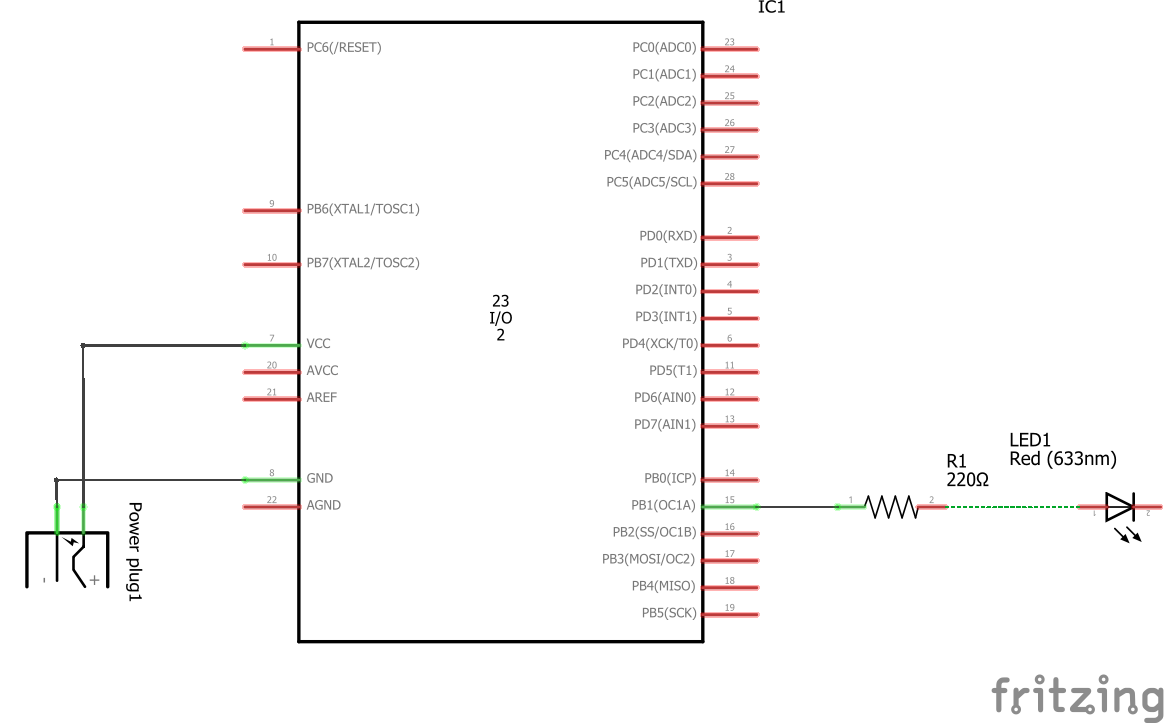
\includegraphics[scale=0.8]{SleepMode_esquematico.png}
 \fautor
\end{figure}

\begin{figure}[htb]
 \caption{Montagem: Sleep Mode}
 \label{fig:Montagem: Sleep Mode}
 \centering
 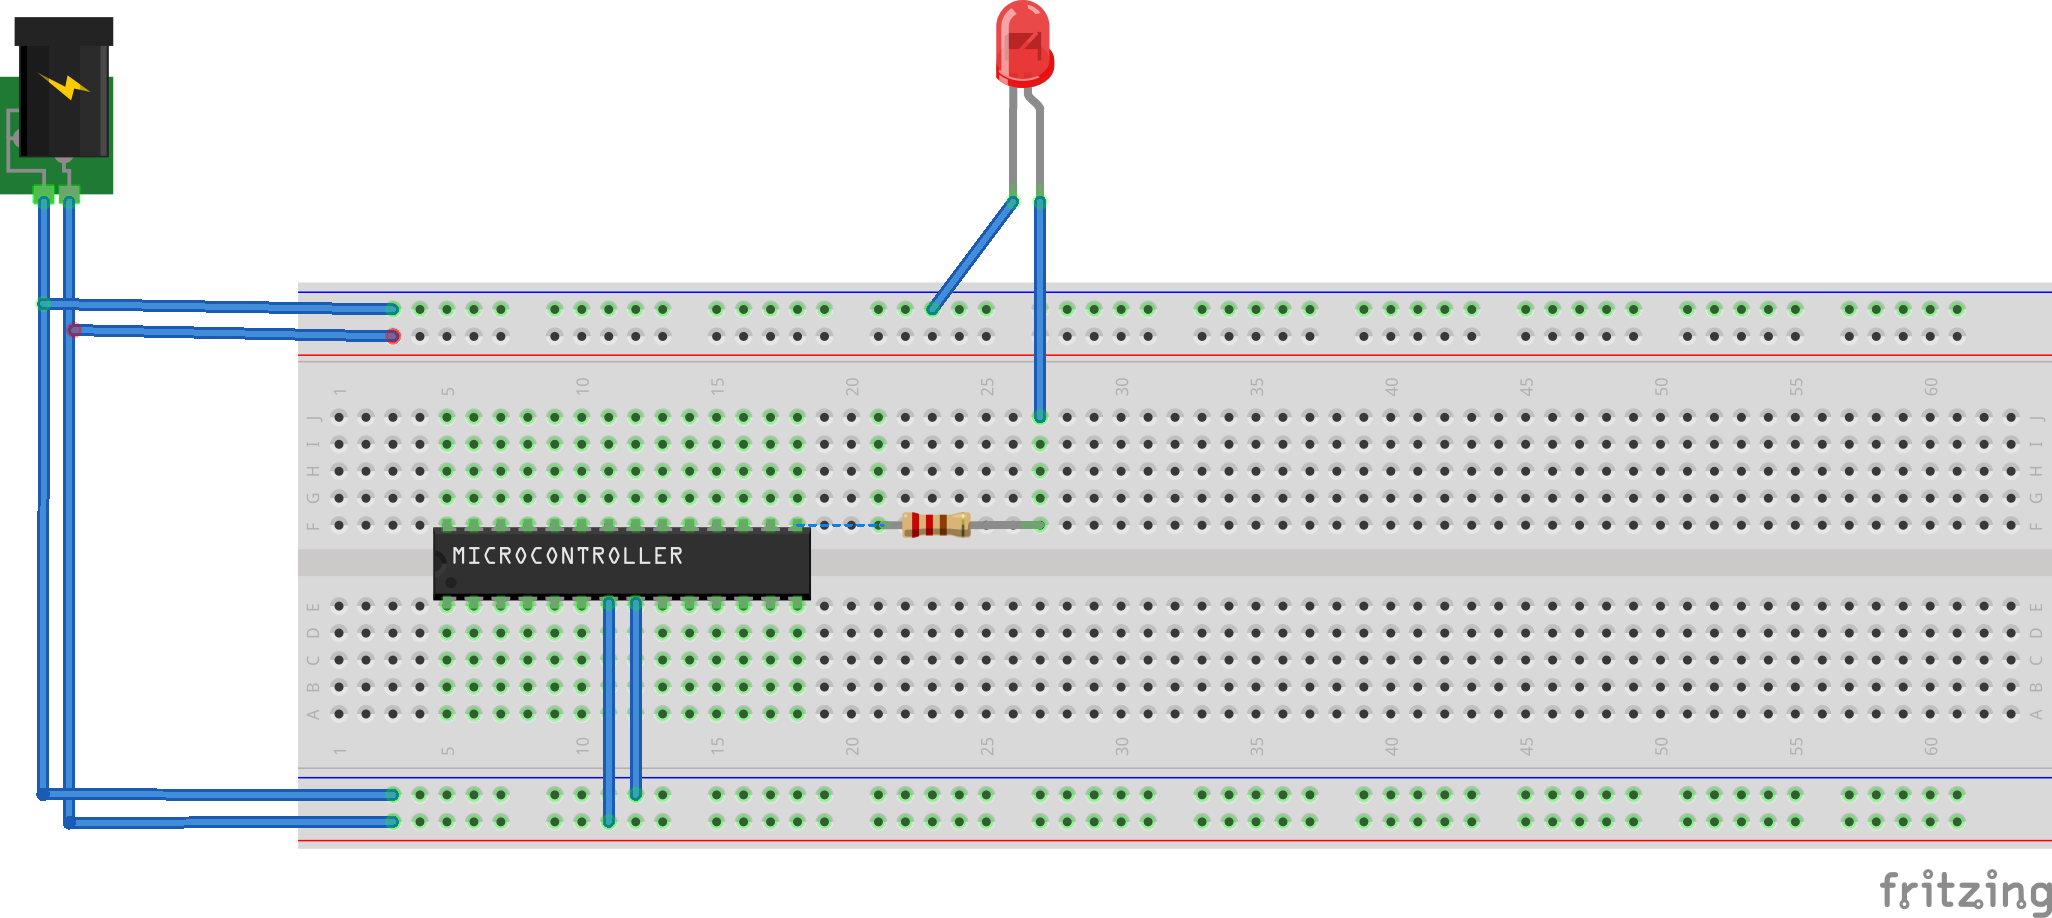
\includegraphics[scale=0.8]{SleepMode_montagem.png}
 \fautor
\end{figure}

\begin{codigo}[caption = {Led On/Off in Sleep Mode}, label={codigo: Led On/Off with Slep Mode},language=C, breaklines=true]

 
 /**************************************************************************
 *      Led On/Off - Utlizando Sleep Mode
 *
 * Universidade Federal de Goiás
 * Microcontrolador Utilizado: AVR ATMega8
 * Grupo: Marco Túlio / Vitor do Vale Bernardo / Pablo Silva
 * Descrição: Ligar e desligar um LED utilizando o modo sleep.
 * 
 ************************************************************************/

#include <avr/io.h>
#include <avr/sleep.h>
#include <avr/interrupt.h>
#include "util/delay.h"

int main(void)
{
	DDRB = 0xFF;

   // infinite main loop
   while (1)
   {
	
	PORTB = 0x01; //  Liga Led na porta 01
	_delay_ms(2000); // Espera 2 segundo
	set_sleep_mode(SLEEP_MODE_PWR_SAVE);
	cli(); 	// desligar interrupções
	sleep_enable();	 // Ativa o Sleep Mode
	sei(); //Liga as interrupções
	sleep_cpu(); 
	cli();
	_delay_ms(5000);
	sleep_disable();
	sei();
	
   }
   
}

\end{codigo}